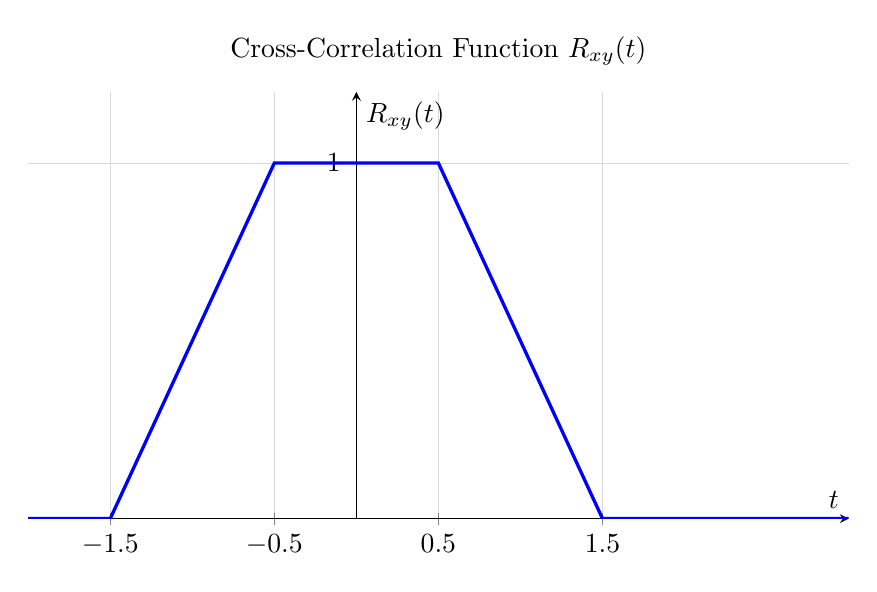
\begin{tikzpicture}
	\begin{axis}[
		width=12cm,
		height=7cm,
		title={Cross-Correlation Function $R_{xy}(t)$},
		xlabel={$t$},
		ylabel={$R_{xy}(t)$},
		axis lines=middle,
		xmin=-2, xmax=3,
		ymin=0, ymax=1.2,
		xtick={-1.5, -0.5, 0.5, 1.5},
		ytick={1},
		grid=major,
		grid style={line width=.1pt, draw=gray!30},
		]
		\draw[blue, very thick]
		(axis cs:-2,0) -- (axis cs:-1.5,0) -- (axis cs:-0.5,1)
		-- (axis cs:0.5,1) -- (axis cs:1.5,0) -- (axis cs:3,0);
	\end{axis}
\end{tikzpicture}